\subsection{Approach}
\writer{Albert}

\label{sec:approach}

This section presents our approach to the project. We have implemented a \textbf{multi-agent} infrastructure
based on a Beliefs - Desires - Intentions model. The defined domain is \textbf{problem specific} and thus
several environment specific \textbf{pre-analyses} are done to reduce the complexity of the problem during
running. Complex goals are handled by decomposing them in simpler ones using \textbf{hierarchical planning}.
For each task, a plan is then computed using \textbf{forward state search}. Moreover, \textbf{specific
heuristics} have been developed for each of the tasks. The system is multi-agent and each of the agents plans
for its own goals and cooperates with the others. In order to solve conflicts, \textbf{merging of plans} by a
central entity has been implemented, although for cases where it is not feasible, \textbf{conflict-solving}
replanning together with \textbf{inter-agent communication} is then used. Details regarding each of these
aspects are presented in the following sections.

Our system implementation has been developed in Java. Due to the nature of the project, where processing time
has to be radically reduced due to the size of the level maps, throughout the implementation we have used a
multitude of data structures and low-level optimization. This has made the state expansions, heuristic
computations and all the required processing as fast as possible.

\subsection{Architecture}
\writer{Cosmin}

% Architecture subsection content

As mentioned in subsection~\ref{sec:approach}, we are using a multi-agent infrastructure, with a central
entity that handles the communication between agents and all the synchronisation issues. A diagram showing the
most important components in our implementation can be seen in Figure~\ref{fig:architecture}.

\begin{figure}[htb]
\begin{center}
 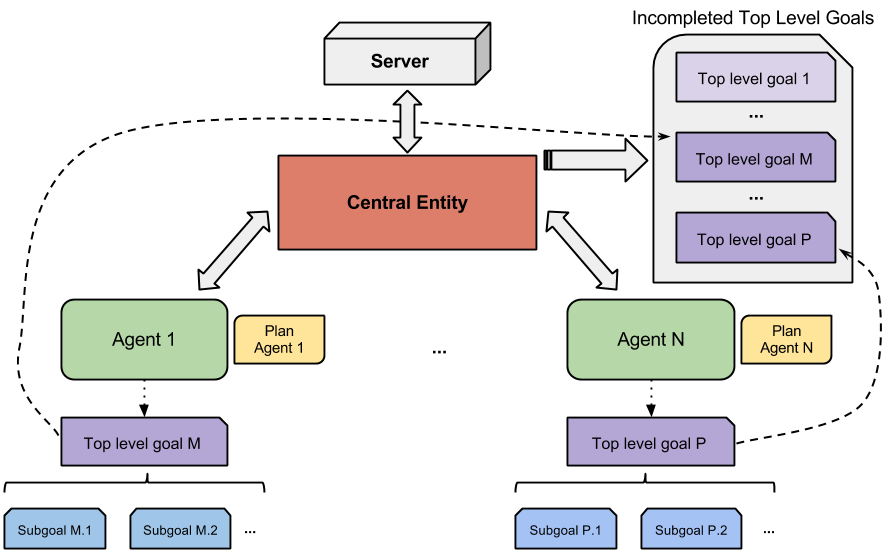
\includegraphics[width=0.92\textwidth]{figures/architecture.png}
 \caption{General system architecture}
 \label{fig:architecture}
\end{center}
\end{figure}

As it can be observed from the figure, the system's main components are a central entity and a set of agents.
The central entity maintains a set of top level goals that need to be completed for a level to be solved. Each
of the agents gets assigned one of these goals and is responsible for breaking it into smaller and easier
subgoals and for elaborating a plan to complete it.

The central component of our application is depicted as the \textbf{Central Entity}. Among the tasks that are
handled by it we can enumerate:

\vspace{-12pt}
\begin{itemize}
\setlength{\itemsep}{0cm}
\item coordinate the communication between the agents
\item manage the list of top level goals that need to be completed
\item decide which agents work on which goals (in situations when multiple agents have proposals for the same goal)
\item merge agents' plans, if possible
\item coordinate the communication between agents when plan merging conflicts appear
\item handle communication with the server
\end{itemize}
\vspace{-0.3cm}

Each of the agents in the system handles the following tasks:

\vspace{-12pt}
\begin{itemize}
\setlength{\itemsep}{0cm}
\item make proposals for each of the goals it can handle
\item divide the goals into easier subgoals
\item make a plan for completing its goal
\item make a plan to solve a plan merging conflict, if needed
\end{itemize}

\vspace{-0.3cm}
\begin{figure}[!htb]
\begin{center}
 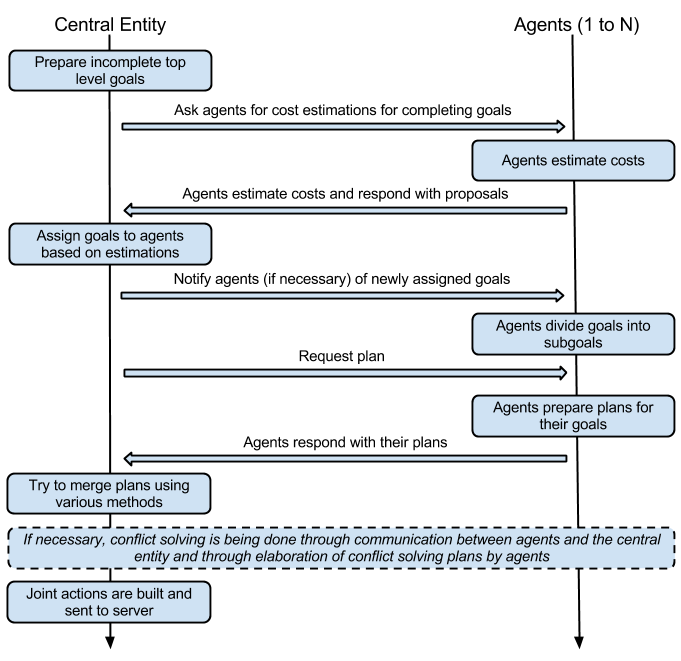
\includegraphics[width=0.75\textwidth]{figures/communication_flow.png}
 \caption{Brief representation of important steps and communication flow}
 \label{fig:communication_flow}
\end{center}
\end{figure}

Figure~\ref{fig:communication_flow} shows the most important steps followed by our implementation and the
communication flow between the agents and the central entity. The diagram only depicts a full iteration of the
steps and it has to be mentioned that, while running, some of the steps and communication messages might not
be applicable or are skipped for optimization reasons. More details about these optimization will be provided
in the following subsections.

Initially, the central entity is identifying the top level goals that still need to be completed.
Subsequently, agents are asked to compute an estimation of the cost of the plan for solving those goals (if
applicable). Based on these estimations, the central entity then assigns goals to the agents. After this step,
agents break down the goals into subgoals that are easier to use and for which different heuristics can be
applied and then use an AStar-based search to identify a plan. These plans are then connected by the central
entity, which tries to merge them using various methods. If the merge is successful, the joint actions are
extracted and sent to the server for each turn. If the plans for some of the agents cannot be merged, the
conflicts are solved under the coordination of the central entity. All these steps and the actual
implementation optimizations are presented with more details in the following subsections.


\subsection{Techniques}

\subsubsection{Preanalysis}
\writer{Albert}
As identified in Section~\ref{sec:problem}, an early analysis of the map could provide valuable information to
be used by the agents when exploring states. For example, using the Dijkstra distance instead of Manhattan
improves the correct choice of goals. Therefore, after initializing the map, the following analyses were
precomputed for further use by the agents. The first step consisted in creating an initial graph, where
vertices are the cells and the edges represent the links to their respective neighbours.

\paragraph{Dijkstra distance}

In order to provide the agents with the most accurate approximation of the real distance between two cells, we
considered that the best approach was to use \textit{Dijkstra's algorithm}, which is a graph search algorithm
that computes the shortest path distance between a cell (vertex) and every other cell.

With this solution, we were able to make the agents go for the closest \textit{accessible} goal. When using
the Manhattan distance, the agents go for a goal which is falsely considered to be closer, although there are
walls in between and the real distance is larger.

We have found, however, that for certain maps which exceed a certain dimension, the analyses is
computationally very expensive and the time consumed by the computation of Dijkstra's graph is too large or
contains too many free cells. For these maps, in order to be able to complete them within the maximum time of
the competition, we decided that we would use Manhattan distance instead.

\paragraph{Betweenness Centrality}

The problem analysis also states that identifying the relevant cells in a map is important in order to avoid
blocking them or in order to allow the agents know which goal cells have to be completed first. Therefore,
with the network graph that we had previously built, we could use a measure such as the betweenness centrality
of a node. This measure consists of the number of shortest paths from each vertex to all others, that pass
through the evaluated node. In Figure~\ref{fig:hanoi} we present an example of the betweenness centrality
measure for the cells of \textit{Boxes of Hanoi} map. It can be observed that cells situated at the end of
each column had a score of 0, while the top row had the higher scores. Thus, this property can be used in
heuristics for penalising agents that leave boxes in important cells or for determining important goals.

\begin{figure}[htb]
\begin{center}
 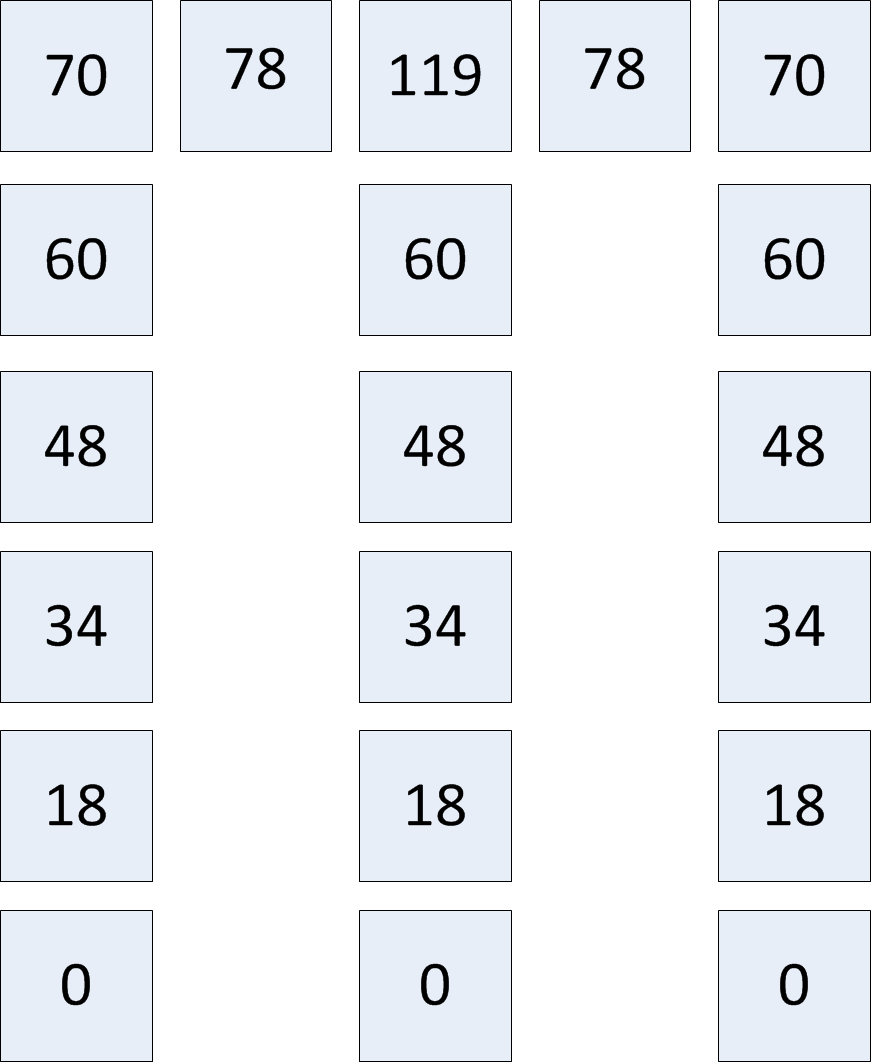
\includegraphics[width=0.3\textwidth]{figures/hanoi.png}
 \caption{Betweenness centrality for the Boxes of Hanoi map}
 \label{fig:hanoi}
\end{center}
\end{figure}

Once again, this is an expensive metric, having a cost of $O(|V|^2log|V| + |V||E|)$. Therefore, for those maps
for which the cost was too large, and thus would make the system not be able to finish on time during the
competition, this property was not computed and a default value was given to all the cells.

\paragraph{Degree Centrality}

Another property that can be easily obtained after building the network graph is the degree centrality, which
is the number of links that a node has\footnote{In our case, the number of neighbours of each cell}. This
measure is useful to identify those cells that, even though they have a high betweenness centrality, also have
many neighbours (4), and thus, should not have as much importance as the ones that could block a path.

\paragraph{Group of goals}

The last analysis that is precomputed is the identification of groups of goals, as for example in
Figure~\ref{fig:goalshanoi}. Being able to recognize groups of goals was defined as crucial, especially in
cases of maps similar to boxes of Hanoi. Therefore, we built an algorithm that for each goal analyzed if there
is any neighbour goal, and recursively, computes the whole group. The usage of these groups permits the agent
to complete first the cells that are part of a group and that have a lower betweenness centrality, meaning the
ones that do not block other goals.

\begin{figure}[htb]
\begin{center}
 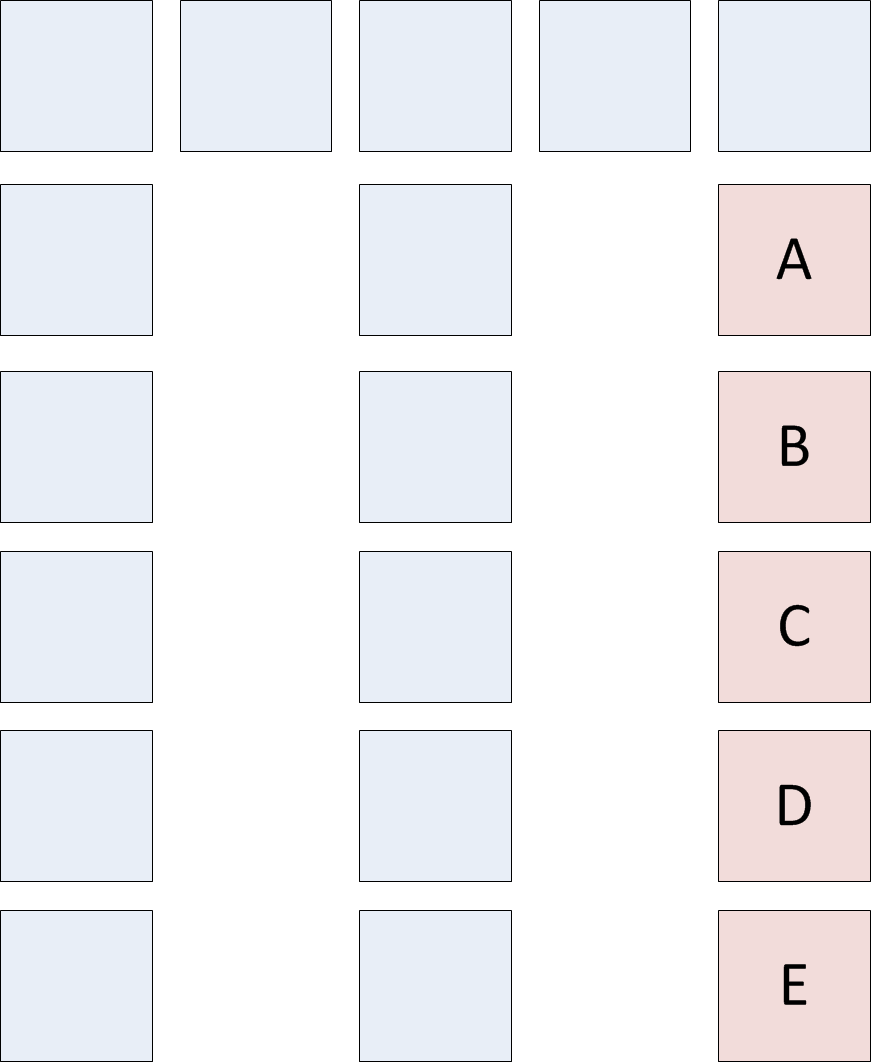
\includegraphics[width=0.3\textwidth]{figures/goalshanoi.png}
 \caption{Identification of groups of goals cells}
 \label{fig:goalshanoi}
\end{center}
\end{figure}


\subsubsection{Goal picking}
\writer{Albert}
As stated, one of the major challenges was to properly select the goals correctly, especially the order in
which they were going to be completed; choosing an incorrect order could lead to an unresolvable state.

In our architecture, the Central Entity is responsible for computing all the top level goals needed to be
completed by the agents and for asking the agents for an estimation of the cost that would require them to
complete each goal.

For computing this cost, specific heuristics for each top level goal were designed. For instance, for the
\textit{DeliverBoxGoal}\footnote{The top level goal saying that a particular box has to be delivered to a
particular cell}, the following properties were taken into account, with different importance:


\vspace{-12pt}
\begin{enumerate}
\setlength{\itemsep}{0cm}
    \item Distance (Dijkstra/Manhattan) between the agent, the box, and the goal.
    \item Betweenness centrality of the cell in which the box was.
    \item Distance from the goal cell to other boxes.
    \item Betweenness centrality of the goal cell.
    \item Blocking another goal by solving this one.
    \item Undoing a goal.
\end{enumerate}
\vspace{-0.3cm}

Choosing the correct value is a complex issue: giving too much importance to one of the properties would mean
that others might not even be able to influence the final score. There are two of them that are penalized with
a high value: blocking other goals and undoing goals. Also, goals situated in cells with lower betweenness
centrality are considered to be better alternatives if possible to use, so it was important to penalize the
rest.

% SHOULD WE ADD THE FORMULA??

\subsubsection{Exploration}
\writer{Rafaela}
State exploration is necessary in order to determine the best possible alternative an agent has for achieving
its goal. Our project tackles the exploration problem by using the A-Star approach together with various types
of heuristics which depend on the types of goals, the results of the pre-analysis of the map, etc. (the
heuristics are described in Section \ref{sec:heuristics}). This approach enables the finding of the path
closest to the optimal solution.

\subsubsection{State}
\writer{Ruxandra}
As the A-Star algorithm used to explore the states for each agent can expand a very high number of states, we
need to take care what we include in a state. A state is defined by the configuration of boxes on the map as
well as the agent for which the state is calculated. We chose to ignore the other agents when doing state
expansion, as taking them into account would not be useful for our purpose. Everything else related to the map
was kept in a separate, common resource.

Even though we try to keep as little information as possible in a state, for large maps with high number of
boxes, we still encountered memory problems. To solve this, we kept all the references to the boxes in the
common resource and used only indexes to cells and boxes in the actual state. Furthermore, to know which cells
are occupied we used a BitSet to save space and speed up computations.

However, in the expansion we noticed that, in some situations, the algorithm was expanding slower than it
should have. After doing some testing we have realized that for a high number of states, the collisions
between the hash-codes\footnote{Used in various types of data structures} of the states would be very high.
This is why we implemented our own hashing method for the states. For optimality reasons, when creating a new
state based on a previous state, we used the hash of the previous state to which we add/ subtract values
depending on the differences between the two states (boxes' positions/ agent's position). This optimization
helped in expanding the states faster as it is easier to compute the hash, but also because the hash is better
suited for the problem and gives fewer conflicts.

\subsubsection{Plan merging}
\writer{Rafaela}
\label{sec:plan_merging}

In multi-agent systems, as mentioned in the \ref{sec:architecture} section, one of the most important aspects
to be considered is how plans originating from multiple agents are merged together, so that no actions are
conflicting and that no resources are used at the same time.

Our approach to plan merging is to find whether there is an optimal way to intercalate the agents’ actions in
order to avoid illegal situations\footnote{For example, when 2 agents try to move in the same cell or push the
same box}, possibly delaying the actions of some of the agents. Our aim is to offer an optimal plan merging
solution, in case such a plan merging is possible. A plan merging fails when, no matter the number of NoOp
actions that one or multiple agents perform, a solution for all of them to achieve their respective goals is
impossible.

Two alternatives were considered for merging multiple plans. The first one was to merge all the agents' plans
into one plan at once. The second solution was to merge the plans one at a time: the first plan with the
second one, then the result with the third one and so on. After analysis, we have agreed that the best option
for us is to try to merge the plans of all active agents (agents that have goals) at the same time. This
decision is supported by the fact that, in this way, it is easier to identify which agents’ plans collide. In
the second option of merging the problem is that identifying which agents have conflicting actions is almost
impossible after we have already computed a merged plan for other agents.

For trying out all possible solutions of merging the agents’ plans, we are using an algorithm based on
backtracking, that loops through all options of intercalating agents’ possible actions. At each step, it tries
to fit as many possible actions from the agents’ plans and delay the other actions. Furthermore, the states
that result after applying a set of actions are only computed (expanded) when and if is necessary, for
optimisation reasons.  An example for how the algorithm works for three agents is shown in Figure
\ref{fig:plan_merging} \footnote{The red colored option is generated but cannot be used due to incompatible
actions, the green option is valid so can be expanded while the grey nodes are not even generated or expanded.
The dash displayed in some nodes represents that a NoOp action has been introduced for the respective agent.}.

\begin{figure}[htb]
\begin{center}
 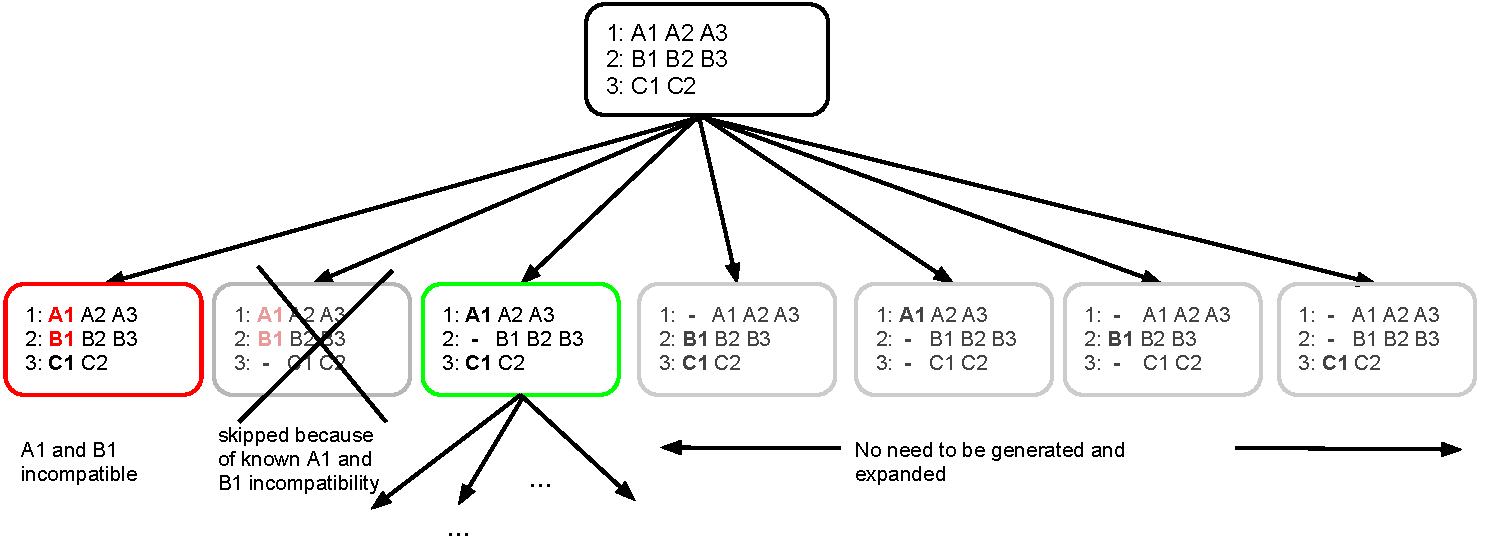
\includegraphics[width=\textwidth]{figures/plan_merging.pdf}
 \caption{Tree for merging}
 \label{fig:plan_merging}
\end{center}
\end{figure}

As it can be seen in Figure \ref{fig:plan_merging}, when we try to merge plans for all three agents, we have
an incompatibility between actions from agents 1 and 2 (actions A1 and B1). The backtracking algorithm will go
back and try other options. For optimisation reasons, our algorithm does not even try to expand the second
option (having active agents 1 and 2 and give agent 3 a NoOp action), because we already know from the
previous try that agents 1 and 2 cannot be active at the same time at this point. The algorithm moves to the
following option and tries to keep the actions from agents 1 and 3 while agent 2 has a NoOp action. This, for
the assumed case, works and the backtracking algorithm will move forward to analyse the next actions remaining
for all agents in a similar way. Assuming that the algorithm will find a solution on this branch, all the
following possibilities from this level (activating agents 2 and 3, or just agent 1, or just agent 2 or just
agent 3) are not even generated (not to mention expanded). This approach saves a lot of resources of time and
memory.

Another optimisation we brought to this algorithm is that we pre-generate lists with all possible options of
activation for agents. The lists contain true or false depending if the agents can perform their action or
have a NoOp action at a certain level. Since we pre-generate and save these options, there is no need to
generate them each time we move to a new level in the options’ graph with the backtracking algorithm. Also,
the options are sorted so that if a merging is possible, one that is closest to the optimal situation is
found.

We have also taken into consideration the fact that usually, not all agents will need to merge their plans. It
is more common to have groups of agents needing to access common resources (boxes or cells) and, thus, needing
to merge only the plans they have. We have taken this into consideration in our solution and we keep track of
groups of agents that need to use, at one point in their plan, the same resources as other agents. In case
there are agents who do not have anything in common with others, their plans will automatically be done, the
merge with other plans not being needed. Also, merging between groups is not needed.

For example, in Figure \ref{fig:no_merge}, considering agents 0 and 1 need to access boxes A and B
respectively and that agent 2 needs to access box C, we would need to merge the plans of agents 0 and 1, but
agent 2 can simply go on with its own as it is not interfering with anyone's plan at any moment. Thus a
merging of plans is only done for the ones of agents 0 and 1.

\begin{figure}[htb]
\begin{center}
 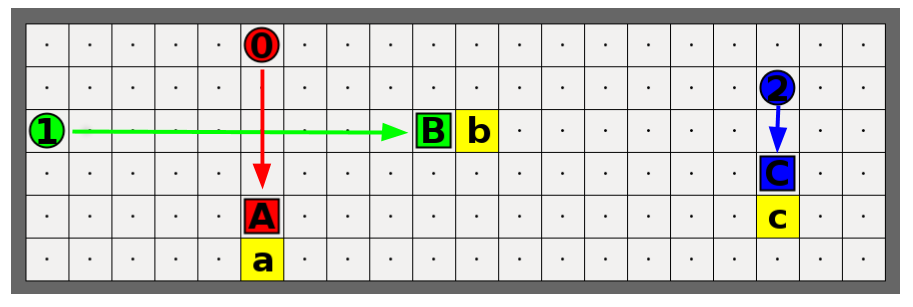
\includegraphics[width=0.8\textwidth]{figures/no_merge.png}
 \caption{Agent 2 does not need a plan merge}
 \label{fig:no_merge}
\end{center}
\end{figure}

\subsubsection{Plan merging conflict identification and solving}
\writer{Rafaela, Cosmin}

While merging plans, there are some situations where plan merging cannot possibly be made, even though all
possible plan intercalation ways are tried. We have called this plan merging conflict.

In order to make a good decision on how to solve such situations, we first need to identify them in a correct
way. In some situations, they can even be identified even before running the merging algorithm. On way in
which we have identified the apparition of a conflict is by analyzing if the paths of two agents are
colliding. Two paths collide if the end or the beginning of an agent’s path (that it has to follow in order to
complete a goal) is situated on another agent’s path and the two cannot avoid each other no matter how many
NoOp actions they might do in order to try to merge their plans.

When a conflict is found\footnote{Either though the above mentioned method or simply because plan merging
fails}, agents need to solve it in order to be able to achieve their goals. The conflict solving can be done
by the central entity, it can be discussed between the conflicting agents or a hybrid solution can be used. In
our approach, we have considered the hybrid solution, in which the central entity is the one identifying the
conflicting situation, but then it contacts the agents so that they can come up with possible solutions for
solving the conflict. The steps of our plan conflict solving process can be seen in
Figure~\ref{fig:conflict_solving} below.

\begin{figure}[htb]
\begin{center}
 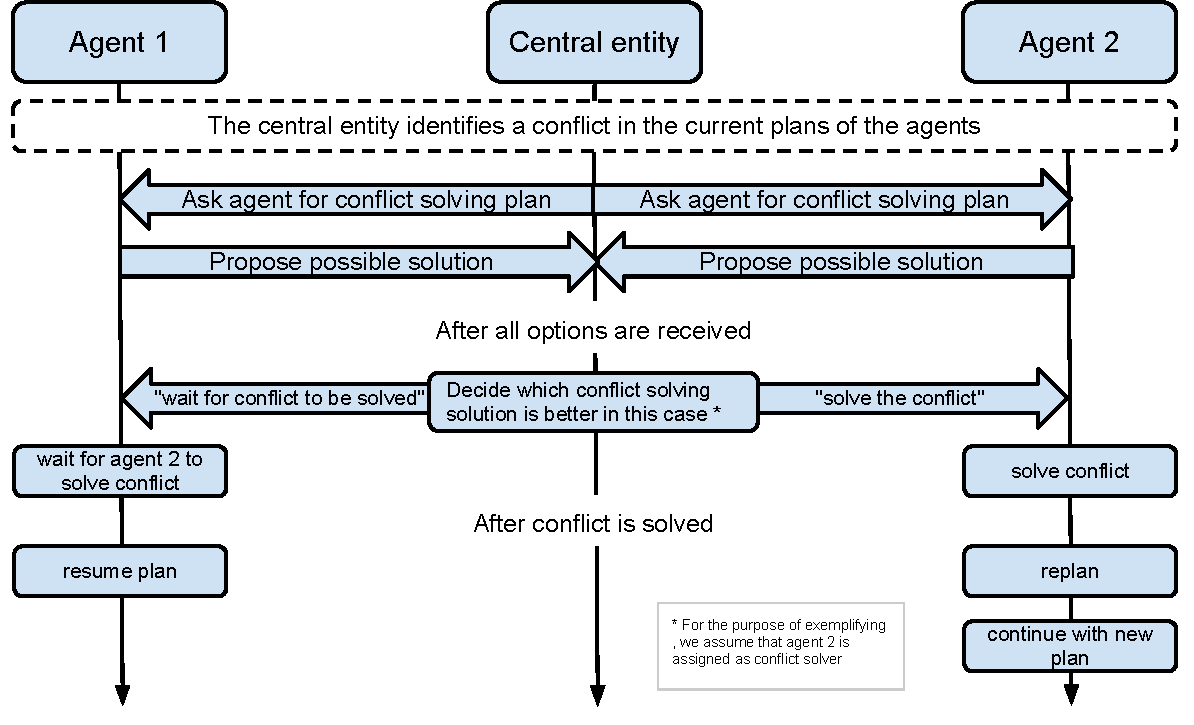
\includegraphics[width=0.7\textwidth]{figures/conflict_solving.pdf}
 \caption{Identifying and solving plan merging conflicts}
 \label{fig:conflict_solving}
\end{center}
\end{figure} 

Basically, the central entity will notice that there is a conflict based on the plans the agents submitted.
Identifying this, it will send a notification back to the agents asking them to propose a way to solve the
problem. Both agents compute their own solution for solving the conflict and send it back to the central
entity. The central entity can then decide, based on the costs of the solutions, which of the agents should
work on solving the conflict and which will need to wait for the other to finish its conflict solving plan
before resuming its initial plan. In the given example, agent 1 will wait for agent 2 to solve the conflict
and then agent 1 can resume its original plan. Agent 2 now needs to re-plan and see if it resumes the initial
plan (if it’s the best option) or if it chooses another goal which will lead for it to have a new plan.

Similarly to the case presented in Section \ref{sec:plan_merging}, when two agents are conflicting and there
are other agents who are not, there is no need to make the agents which are not in conflict wait for the
conflict to be solved before they can continue their plans. However, in the case that the plan chosen to solve
the conflict affects the plans of other agents (which were not originally in the conflict), then, plan merging
or conflict solving is tried for the new affected agents.

\subsubsection{Plan cooperation (clear my path goals)}
\writer{Cosmin}
There are cases when agents cannot solve some situations or some goals by themselves, thus cooperation between agents is required. One such situation is presented in figure \ref{fig:cooperation}. As we can see, agent 0 is not able to reach box A in order to deliver it unless box B is moved out of its path. For this, agent 0 first detects that he cannot reach box A, then it identifies that box B should be moved out of the way. After this, other agents are asked to clear the path and agent 1 comes up with a plan to move B out of the way and return to its initial position. After this, the central entity merges the plans of the 2 agents and the solution is found.

\begin{figure}[htb]
\begin{center}
 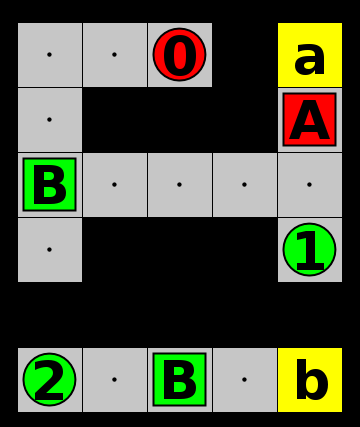
\includegraphics[width=0.35\textwidth]{figures/cooperation.png}
 \caption{Situation where agent cooperation is needed}
 \label{fig:cooperation}
\end{center}
\end{figure}

Thus, as identified from the situation above, the first thing that needs to be done is to identify when an
agent cannot fulfil its goal (in our example, agent 0 cannot reach box A). For this, we are first performing a
normal exploration looking for a solution. If no solution is found, we perform a second search starting with a
‘virtual’ state where boxes that cannot be moved by the agent are removed. If there is any way for the agent
to reach its goal, it will be identified in this second search and the boxes that block the path are
identified.

The second aspect needed to resolve scenarios such as the one presented above is how other agents are asked
for cooperation. In our system this was tackled based on the existing goals assigning/resolving
infrastructure. When an agent needs a path cleared, it communicates with the central entity which, in turn,
introduces a special type of Top Level Goal into the system. This is then handled like every other
goal\footnote{As mentioned in section \ref{sec:architecture}}: agents make estimations for the cost of solving
it, one of the agents gets assigned to work on it and then comes up with a plan. In the scenario above, only
agent 1 will come up with a goal solving cost estimation (as agent 2 cannot even reach box B) and will get
assigned to solve it.

\subsubsection{Partial observability}
\writer{Cosmin}

Our implementation is handling partial observability by identifying when one of the actions that was sent to
the server fails. As, due to applicability checks done when expanding states and when merging plans, there is
no possibility that a joint action has failed because of incompatible actions\footnote{E.g. an agent moving a
box in the same cell where there is another agent or another box}, cells which have unknown objects on them
are easily identified. Whenever this happens, our Central Entity is updating the beliefs of all the agents by
marking the cell as occupied in a central synchronized map representation. Further on, all the agents whose
plans might be affected by the newly discovered occupied cell are notified in order to replan.

\subsubsection{Heuristics}
\writer{Javier, Marius}
\label{sec:heuristics}

As previously stated, the A-Star search we used is guided by various heuristics, depending on what the current
subgoal is. Different heuristics were designed for having an agent get near a box or for having him move that
box.

For both types of goals, the heuristic takes into account the following: distance from the current cell to the
cell of the box, if the agent pushes or pulls another box, if the agent leaves boxes in cells with high
betweenness centrality, if the agent leaves boxes in other goal cells, if the agent blocks the access to other
goal cells, if the agent undoes a satisfied goal or if the agent pushes or pulls in a dead-end corridor.

A score is given for each of the measures and conditions mentioned above. These scores are multiplied by a
coefficient and added, resulting in the final heuristic score.

Depending on the type of the map, the values of the coefficient of each term is changed, thus resulting in
different heuristics for different types of maps.

For getting next to a box, the distance is the most important factor to be considered, as we usually want the
shortest path. However, if that shortest path is through another cell which has a satisfied goal, due to the
penalty for undoing goals, the computed path detours that cell, trying to find a better option according to
the cost of the path.

For moving the box to its goal cell, the agent is penalised, for example, for pulling in a dead-end corridor.
In Figure \ref{fig:heuristics1}, the agent needs to push box C to its goal, because if it pulls it, it would
be stuck in a dead-end and it would have to move box C from its goal, in order to be able to get out.

\begin{figure}[htb]
\begin{center}
 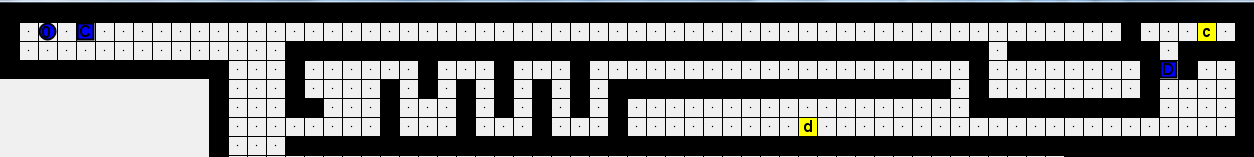
\includegraphics[width=0.8\textwidth]{figures/heuristics1.png}
 \caption{In this case, agent 0 needs to push box C to the goal, not pull it.}
 \label{fig:heuristics1}
\end{center}
\end{figure}

%something about hanoi? Javier? :D %

In some situations it is impossible to reach the box that the agent wants to deliver because there are some
other boxes blocking its path. In this situations it is necessary to clear the path for the agent. Figure
\ref{fig:heuristics2} shows a hanoi-like map, where the agent wants to deliver box A but the path is blocked
by other boxes and there is also a dead-end corridor.

For clearing the path the agent uses the dead-end corridors for storing the boxes that are in the middle of
its path. The final cell of each box is determined by the deepness of the dead-end. This means that the box is
pushed in the same direction while the betweenness centrality of a neighbour cell is lower than their own.

Another fact that it is necessary to take into account is that the first cell of the corridor must be empty,
in case that the agent needs this cell to make some turn movement, if it needs to change from pulling to
pushing.

\begin{figure}[htb]
\begin{center}
 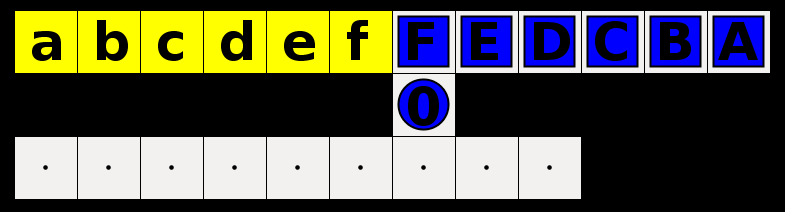
\includegraphics[width=0.6\textwidth]{figures/heuristics2.png}
 \caption{Hanoi-like map}
 \label{fig:heuristics2}
\end{center}
\end{figure}